\section{Performance of WR Transparent Clocks}
\label{sec:issues}
This section examines the features of WR TC that are commonly~\cite{biblio:tc_perf} taken in to
account for the estimation of the performance of a TC: 
\begin{itemize}
    \item Accuracy and precision
    \item Correction factor stability
    \item Maximum update rate
    \item Rapid reconfiguration after topology changes
\end{itemize}


\subsection{Accuracy and precision}

%\subsubsection{WR TC Peer to Peer}
%The chapter ~\ref{sec:wr} resumes how WR accomplish
%sub-nanoseconds synchronization and picoseconds jitter. It is based on the
%acharacterization the asymmetries of the link a priory, and a clock lookback
%technique. By doing this WR is able to  enhance the timestamps on ingress ports. 

The performance of the WR Peer-to-Peer TC prototype is compared in this section
with the WR BC. For this purpose, the pulse per second (PPS) skew between a WR slave clock 
connected to a WR master clock using up to 5 WR switches is measured.
\figurename~\ref{fig:test_setup} shows the setup used for the benchmarking. 
The WR master and slave clocks are Exploder cards
~\cite{biblio:wr_gsi} with a modified WR PTP software~\cite{biblio:wrpc-sw}.
The switches are WR v3 with a modified firmware. The WR master and slave
are connected to a Lecroy Waverunner oscilloscope using lemo cables of the 
same length. 

The histograms in \figurename~\ref{fig:wr_bc} and~\ref{fig:wr_p2p} show the outcome of the
measurements.

%\subsubsection{WR TC End to End}
%\begin{figure}[!t]
%%\centering
%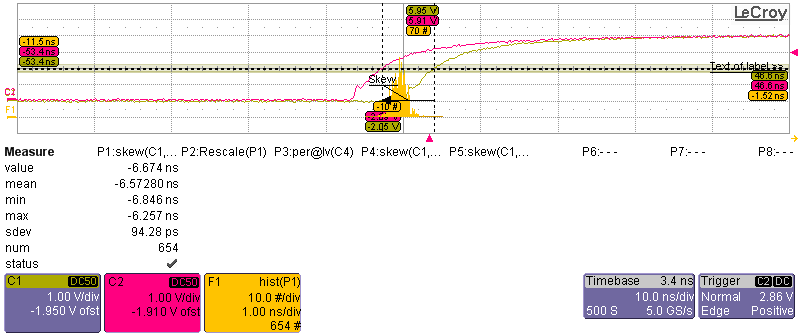
\includegraphics[scale=0.25]{fig/tc_5_switches2.png}
%\caption{WR E2E and P2P Transparent Clocks}
%\label{fig:wr_tc}
%\end{figure}
%
The offset between master and slave is in the range of nanoseconds and
increases with the number of switches in cascade. Since the WR nodes~\cite{biblio:wr_gsi} 
and small form-factor pluggable (SFP) used in this setup haven't been calibrated yet, 
the fixed delays are missing in the
calculation of $delay_{ms}$~\eqref{eq:delayms}. In the case of the TC also
affects to the measurement of the residence time~\eqref{eq:residence_time}. This
explains the difference of almost 1 ns offset between the clocks, as well as
the increment of the offset as the number of TCs in the topology increases.

The standard deviation, $\delta^2$, of the PPS skew in the TC is almost constant, 
while in the BC increases as the number of BC increases. 
This result shows that the WR model is also applicable to TC even though the
phase measurement and the time stamp enhancement~\ref{sec:delay_ms} is not done between master and
slave clock, but between TCs or slaves. 

\FloatBarrier
\begin{figure}[!t]
\centering
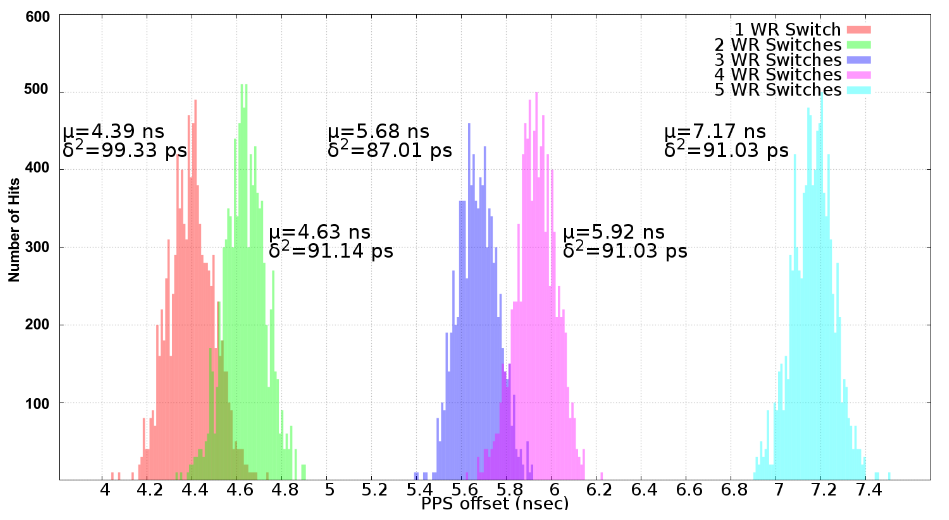
\includegraphics[scale=0.29]{fig/p2p.png}
\caption{Histogram of PPS offset between WR Master, up to 5 WR TC Peer-to-Peer and WR Slave}
\label{fig:wr_p2p}
\end{figure}

\subsection{Residence Time Stability and Maximum Update Rate}

Both, maximum update rate and residence time, are features greatly influenced
by the latency in the TCs. As a result, the synchronization could suffer
performance degradation. 

An increment of the residence time in a TC is normally associated 
to an increment of the traffic in the switch. The authors of ~\cite{biblio:tc_perf} 
present the parameter \textit{Correction Factor Error} (CFE). It expresses the difference 
of the latency measured by a test equipment and TC under test. The origin of this error in 
the measurement of the residence time is implementation-dependent, and it can be associated 
in the most of the cases with delays in the input or output queues of the switch.

During the acquisition of measurements for this paper, the residence time in the
WR TCs has been constant. The propagation delay from master to slave 
minus the residence time in every TC, has only varied in the range of
picosecond in successive samplings. The reason lies in the design of the
hardware in charge of the timestamping~\cite{biblio:tomas} and
deterministic packet forwarding. The WR switch generates the timestamps after 
the output queues. Thereby, the non deterministic delay
introduced during the queuing is already measured in the residence time and the
CFE should be negligible. Besides that, WR switches provide deterministic packet forwarding making use of a 
quality of service (QoS) prioritization scheme and cut-through
switching~\cite{biblio:switch_book}. The traffic tagged as highest priority will be forwarded 
without a maximum delay. The rest of the traffic will follow a queue scheduling algorithm and
store and forward switching~\cite{biblio:switch_book}.

The \textit{Update Rate} (UR) of a two-step clock, is defined as the delay between the transmission of a Sync
message from the master till the reception of the Follow Up message by the slave. 
According to~\cite{biblio:tc_perf}, delays around $10-30\%$ of the Sync interval can create
instability in the slave. 

\FloatBarrier
\begin{figure}[!t]
\centering
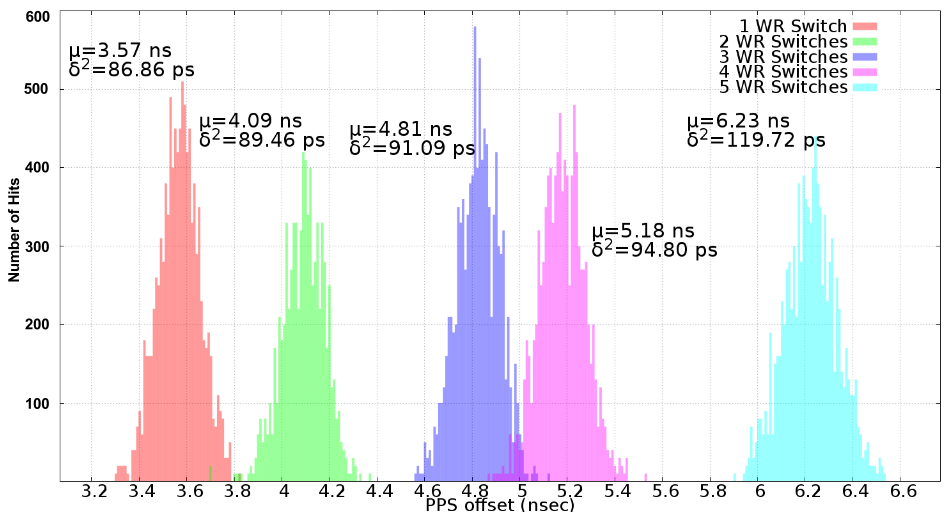
\includegraphics[scale=0.29]{fig/bc.png}
\caption{Histogram of PPS offset between WR Master, up to 5 WR BC and WR Slave}
\label{fig:wr_bc}
\end{figure}

\figurename~\ref{fig:update_rate} shows the average, maximum and minimum delay between SYNC
transmission and FOLLOW\_UP reception in topologies up to 5 layers of TC. Since
the processing of the Sync packets flow, in WR TC, is done in software, the
delay is in the range of milliseconds, and the ratio between the UR and the
SYNC rate, $1 Hz$, is between $10-20\%$. Despite that, the measurements in
\figurename~\ref{fig:wr_p2p}, show a stable and tight synchronization of the
slaves to the master.

\FloatBarrier
\begin{figure}[!t]
\centering
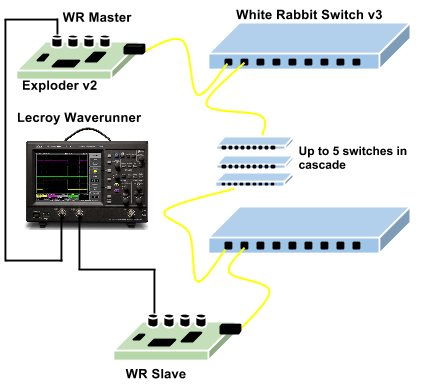
\includegraphics[scale=0.50]{fig/tc_test_bed.png}
\caption{Test setup}
\label{fig:test_setup}
\end{figure}


\subsection{Reconfiguration after Topologies Changes}

A timing system application, often, demands not only accuracy and precision, 
but also stability and continuation of the synchronization in the events
of failure. As an illustrative example, the new timing systems for GSI and CERN,
based on WR technology, require a high stability of the synchronization. 
Both timing systems achieve resilience against 
network failures using redundant connections.  Lower layer protocols stablish a
spanning tree topology setting ports connected to cyclic paths to block/passive
state. In this case only the Peer-to-Peer TC still issues the synchronization between the
ports in both directions. As a result, both clocks have the link delay
information. This offers the possibility of having the link immediately available after 
changes in the topology. Hence the reconfiguration time doesn't depend on the TCs anymore 
but in the lower layer protocol. WRS has already
proposals for implementing a transparent mechanism ~\cite{biblio:wrswitch} for
recovering from single points of failure in a redundant network.

\begin{figure}[!t]
\centering
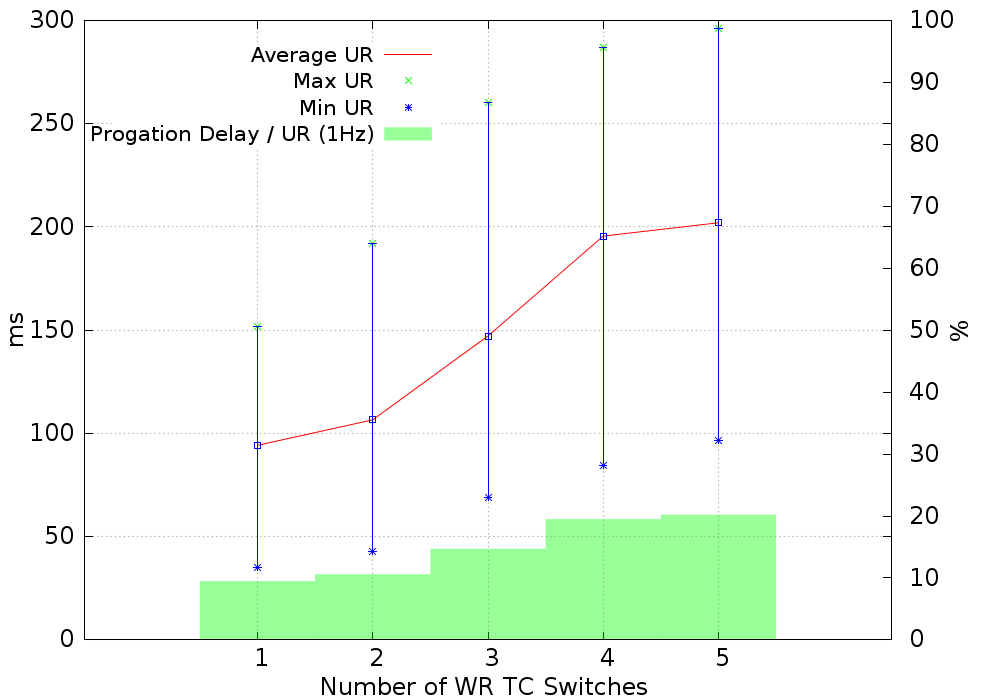
\includegraphics[scale=0.27]{fig/update_rate.png}
\caption{SYNC transmission to FOLLOW\_UP reception delay and Update Rate}
\label{fig:update_rate}
\end{figure}
